\chapter{Hyperfine coupling}
\section{Adatom in the SK-approximation}
While the model of an effective vacancy in the $p_z$ manifold is very simple and useful, it lacks some ingredients that can also provide interesting physical effects.

We are going to discuss briefly here the implementation of this system in a \ac{sk} framework as described in previous chapters. This approximation will provide some insight in the physics of the other orbitals.


The most naive approach would be to use the \ac{sk} parameters detailed in previous chapters (see table~\ref{G_SK_params}). These parameters were calculated for $H$ atoms passivating the edges of graphene nanoribbons\cite{Gosalbez-Martinez2011} where the main hybridization occurs with the $\sigma$ orbitals of graphene. There is no good reason why these hoppings parameters should hold for an adatom on top of flat graphene. For the sake of the argument we will start with those values in order to spot the difference with the idealized one-orbital model, and then proceed to consider the hopping parameters as somehow free parameters that we can tune.


In a first approach we are going to neglect the well known $sp^3$ deformation of the lattice\cite{} and consider simply that the $H$ atom has some hoppings to the $C$ orbitals. Due to the symmetry of the problem, both the $s$ and $p_z$ orbitals will have a finite hopping with the $s$ orbital while de $p_{x/y}$ will not. In the \ac{sk} approximation, the effective hoppings will be governed by the parameters $V_{ss\sigma}$ and $V_{sp\sigma}$.


%
%The Lieb's Theorem holds for bipartite lattices at half filling, which is, indeed, the case of graphene when only $p_z$ orbitals are considered. The inclusion of the other $p$ orbitals does not break the bipartite nature of the lattice since their manifold is disconnected from that of the $p_z$ orbitals, \emph{and their on-site energy is the same}.
%The $s$ orbitals are also disconnected from the $p_z$ manifold but their on-site energy is finite (see \ref{G_SK_params}). This fact breaks the bipartite character of the lattice, nevertheless, the $s$ manifold is far in energy and its hybridization with the $p_{x/y}$ orbitals is strong so the bonding-antibonding states are also far in energy.
%
%
%\red{XXX}
%
%
%It is instructive to compare the spectrum of a big armchair island (22686
%%29526
%$C$ atoms) considering 4 orbitals and a $H$ adatom and the same island with only $p_z$ orbitals and a vacancy.
%
%%~~~~~~~~~~~~~~~~~~~~~~~~~~ FIGURE ~~~~~~~~~~~~~~~~~~~~~~~~~%
%\begin{figure}[h!]
%  \centering
%  \includegraphics[width=0.8\textwidth]{defects/fig/spectrum.pdf}
%  \vspace{-5pt}
%\caption{Low energy spectrum of an armchair island. Left panel shows the spectrum when only the $p_z$ orbitals are considered. Right panel shows the spectrum considering all 4 orbitals $s$, $p_x$, $p_y$, $p_z$}
%\label{spectrum}
%\end{figure}
%\FloatBarrier
%%~~~~~~~~~~~~~~~~~~~~~~~~~~~~~~~~~~~~~~~~~~~~~~~~~~~~~~~~~~~%
%
%Notice in figure~\ref{spectrum} that the in-gap state, marked in red, does not appear at $E=0$ as this system is no longer suitable for the Lieb's theorem. The exact energy at which the in-gap state appear depends on the hopping parameters between the $H$ and the $C$ atoms, mainly on the $V_{sp\sigma}$ parameter.
%
%
%\red{XXX}


When only one orbital per site is considered, graphene is a bipartite lattice. The effective removal of one of the sites results in the appearance of a zero energy state. In fact, Lieb's Theorem\cite{Lieb1989} determines that the imbalance in the number of sites of each sublattice equals the number of zero-energy states: $N_Z=|N_A-N_B|$.

The introduction of more orbitals in the description breaks the bipartite character of the lattice since the on-site energy of $s$ and $p$ orbitals is not the same. Even when, strictly speaking, Lieb's Theorem does not apply, the actual behavior does not change drastically.
Usually, the introduction of an adatom will open a small gap and the states that appear are usually not at zero energy, but they do appear inside the gap. The confinement properties described in~\ref{ch:vacancy} do hold.


\section{Dependence on the parameters}
In~\fref{ingap}a) we show the differences in the spectrum when considering 1 and 4 orbitals per atom. The calculations were carried out by considering a big hexagonal island ($N_C>100000$) with armchair edges (passivated by $H$ atoms when 4 orbitals are considered) and a single $H$ adatom placed in its center.
The main difference is the energy at which the in-gap state appears.
Due to the symmetry of the orbitals and the symmetrical position of the adatom, there are only two finite hoppings, $V_{ss\sigma}$ and $V_{sp\sigma}$, shown in~\fref{ingap}b).
The energy of the in-gap state as a function of both parameters is shown in \fref{ingap}. Notice the strong dependence with the $V_{sp\sigma}$ parameter.

%~~~~~~~~~~~~~~~~~~~~~~~~~~ FIGURE ~~~~~~~~~~~~~~~~~~~~~~~~~%
\begin{figure}[h!]
  \centering
  \includegraphics{defects/fig/Vsss_Vsps.pdf}
  \vspace{-5pt}
  \caption{a) Comparison of the spectrum (sketch) of a graphene island using the vacancy in a one orbital model and an adatom in the \ac{sk} approximation using the parameters in \ref{G_SK_params}. Notice that the in-gap state appears close to the valence band rather than in the middle of the gap. b) Scheme of the hopping processes present in this kind of defects. c) Evolution of the spectrum of an armchair island for different \ac{sk} parameters for the $sp^3$ defect. Notice the strong dependence of the in-gap energy with $V_{sp\sigma}$ especially comparing it with $V_{ss\sigma}$. The dashed lines show the value of the ``naive'' parameters in \ref{G_SK_params}}
\label{ingap}
\end{figure}
%\FloatBarrier
%~~~~~~~~~~~~~~~~~~~~~~~~~~~~~~~~~~~~~~~~~~~~~~~~~~~~~~~~~~~%

It is clear that in order to recover the 1-orbital intuition (in-gap state at $E=0$), we require the limit $V_{sp\sigma}\to\infty$. The position of the in-gap state is the most obvious effect, but the composition of its wave-function can change other properties that we discuss in the next sections.


The experimental value for these parameters is difficult to infer\cite{}, and even \ac{dft} calculations depend strongly on the system at hand, so we will consider a wide range of values and explore the resulting physics.\\



\section{Hyperfine Interaction}
\label{sec:hyperfine}
Functionalized graphene has many interesting properties. 

There is an electronic spin $S=1/2$, and a nuclear spin $I=1/2$ very close in space. A natural question is how big is the interaction between them. In particular, if this interaction were \emph{big enough} and \emph{tunable enough}, the system would have all the necessary ingredients to behave as a single qubit.
This idea follows very closely the Kane's proposal for a silicon based nuclear spin qubit\cite{Kane1988}. In this proposal Kane suggests that it would be possible to use the nuclear spin of Phosphorus dopants ($^{31}P$) embedded in Silicon as qubits. The interaction with the qubits would be mediated by the electronic states bounded to the impurity and it could be tuned via an external electric gate which would shift and deform the electronic cloud around the $^{31}P$ to increase/decrease the hyperfine interaction, effectively switching on and off the interaction of the nuclear spin with the rest of the world.
Similarly using an electric gate between two dopants it would be possible to tune the inter-qubit interactions.
Let us address the ``strong enough'' requirement in the following section, leaving the tunability question for later chapters. 

The hyperfine (HF) interaction arises when we consider the effect of the nuclear spin on the electron.

Apart from the interaction of the electron and the proton with the external magnetic field we have to take into account the interaction between them.

By introducing the potential vector $\vec{A}_{I}$ (corresponding to the magnetic field created by the proton, $\rotac{\vec{A}_{I}}$) in the Hamiltonian and expanding to first order in this potential vector, we get the complete hyperfine Hamiltonian:~\cite{Cohen1977book}
\begin{equation}
H_{hf} = \frac{-\mu_{0}}{4\pi}\left[
\frac{q_{p}}{m_{e}R^{3}}\vec{L}\cdot\vec{M}_{I} +
\frac{1}{R^{3}}\left(3(\vec{m}_{e}\cdot\hat{n})
                      (\vec{m}_{p}\cdot\hat{n})-
                      \vec{m}_{e}\cdot\vec{m}_{p}\right) +
\frac{8\pi}{3}\vec{m}_{e}\cdot\vec{m}_{p}\delta(\vec{R})
\right]
\label{full_HF}
\end{equation}
where $\vec{L}$ is the orbital momentum of the electron, $\vec{m}_{e}$ is the magnetic moment of the electron, and $\hat{n}$ is the unit vector of the straight line joining the proton to the electron.\\

The first term in equation~\eqref{full_HF} represents the interaction of the nuclear magnetic moment with the magnetic field created at the proton by the rotation of the electronic charge. If we are considering $s$ orbitals this term will vanish since all the terms would include a factor like $\bra{n,0,0}L\ket{n,0,0} = 0$, so we will drop this term from the discussion.

The second term represents the dipole-dipole interaction between the nuclear and electronic magnetic moments. Again for a \textit{pure} $s$ orbital this term would vanish as a consequence of the spherical symmetry of the orbital. Nevertheless, because of perturbations (from the crystal or external fields) a contribution from this term may become relevant. \red{review, and check the possible modification of $\mathcal{A}$ due to this geometric deformation}

The third term is the so-called ``contact term'', and it arises from the singularity at $\vec{R}=\vec{0}$ of the field created by the magnetic moment of the proton.
This contact term describes the interaction of the magnetic moment of the electron spin with the magnetic field inside the proton (considered as punctual). Notice that because of the presence of the delta function in this term, it will be proportional to the overlap of the wave function of the electron and the proton. This term will be the main contribution to the hyperfine interaction.\\

For the case of a free, isolated Hydrogen atom and for the $1s$ orbital the calculation of the contact term can be done exactly:
\begin{equation}
H^{contact}_{hf} =
%\underbrace{\frac{-\mu_{0}}{4\pi}\frac{8\pi}{3}\frac{g_{p}\mu_{n}}{\hbar}
%\frac{g_{e}\mu_{e}}{\hbar}}_{\mathcal{A}_{0}} \vec{I}\vec{S}
\frac{-2\mu_0}{3}\frac{g_{p}\mu_{n}}{2}
\frac{g_{e}\mu_{e}}{2} \bra{1,0,0}\delta(\vec{R})
\ket{1,0,0}  \vec{\sigma}_e\vec{\sigma}_p =
\mathcal{A}_{0}\vec{\sigma}_e\vec{\sigma}_p
\label{HF_contact}
\end{equation}
where the notation for the kets is $\ket{n,l,m_{l}}$, with $n$ the so-called principal quantum number, $l$ the orbital angular momentum and $m $the third component of said angular momentum. The hyperfine coupling, $\mathcal{A}_{0}$, takes the value:
%\begin{equation}
%\frac{\mathcal{A}_{0}\hbar}{2\pi} \simeq \SI{1420}{\MHz}
%\end{equation}
%%XXX
%correct?:
%\begin{equation}
%\frac{4\pi\mathcal{A}_{0}}{\hbar} \simeq \SI{1420}{\MHz}
%\end{equation}
%bien definitivo (check appendix~\ref{units_A}):
\begin{equation}
  \frac{\mathcal{A}_0}{2\pi\hbar} = \SI{1420}{\MHz}
\end{equation}
Even when the hyperfine interaction appears with energy units in \eqref{HF_contact}, it is commonly expressed in $\si{\MHz}$, neglecting the $2\pi\hbar$ factor. This is technically an abuse of language but widely used, so we will use it carelessly. For the sake of clarity the units have been detailed in appendix \ref{units_A}.

Notice that the contribution to the hyperfine contact term for $p$ (or higher $l$) orbitals vanishes since the wave functions of such orbitals vanish at the nucleus position, so the factor $\bra{n,l,m_{l}}\delta(\vec{R})\ket{n,l,m_{l}}$ will always be zero.\\

In our case of interest, $H$ adatoms, the hyperfine coupling will be quenched by the occupation of the $s$ orbital of the $H$,
\begin{equation}
  \mathcal{A} = A_0|\braket{\phi_s}{\psi}|^2
\end{equation}
where $\ket{\psi}$ is any of the eigenstates of the Hamiltonian and $\ket{\phi_s}$ is the Hydrogen $s$ orbital.

Of course other orbitals centered at the other atoms would also contribute to the hyperfine interaction (since the wave function does not vanish at the position of the nucleus), nevertheless the \ac{tb} approximation does not offer the tools to deal with the deformation of the orbitals what makes it impossible to estimate the evaluation of the orbitals at the $H$ nucleus and comparison with \ac{dft} calculations show that this effect is not the main one for describing this physics\cite{Ranjbar2010}.

For the case of Si:$^{31}$P the hyperfine coupling in MegaHertz is\cite{Dehollain2014,Kalra2014}
%$4\pi\mathcal{A}/\hbar=58MHz$
%XXX $\frac{\mathcal{A}}{2\pi\hbar} = \SI{58}{\MHz}$ ?????
$\frac{\mathcal{A}}{2\pi\hbar} = \SI{117}{\MHz}$


Since we do not have a reliable estimation of the \ac{sk} parameters of the adatom, we will consider them as free parameters. In \fref{ingap} we saw the evolution of the spectrum as a function of the two \ac{sk} parameters. Here we show both the energy of the in-gap state and the hyperfine coupling as a function of the $V_{sp\sigma}$, the main contributor.

%~~~~~~~~~~~~~~~~~~~~~~~~~~ FIGURE ~~~~~~~~~~~~~~~~~~~~~~~~~%
\begin{figure}[h!]
\centering
\includegraphics{defects/fig/coupling_hyper.pdf}
\vspace{-10pt}
\caption{a) Dependence of the in-gap state arising from a single vacancy in graphene monolayer with the $V_{sp\sigma}$ coupling for different $V_{ss\sigma}$. b) Hyperfine coupling with the $V_{sp\sigma}$ coupling in a H adatom on top of graphene.} % c) Hyperfine coupling modulated by an external electric field in bilayer graphene calculated with the optimal parameters calculated in the monolayer case. These numbers are to be considered as an upper limit for the tunability of $\mathcal{A}$.}
\label{hyperfine}
\end{figure}
\FloatBarrier
%~~~~~~~~~~~~~~~~~~~~~~~~~~~~~~~~~~~~~~~~~~~~~~~~~~~~~~~~~~~%

While the position of the in-gap state does not change a lot with the $V_{ss\sigma}$, the hyperfine coupling does present a significant variance with this parameter. This behavior is expected since the increasing the $s-s$ hybridization would reduce the available $H_s$ weight in the in-gap wave function.

Without a thorough study of these parameters (out of the scope of this work) it is worth noting that there is a range of parameters in which the hyperfine coupling is 




\newpage
\section{A Qubit Idea}


Finally, we can write the complete Hamiltonian for our nuclear qubit as a combination of the previous ones:
\begin{equation}
  H = -g_e\mu_e\frac{1}{2}\vec{B}\vec{\sigma}^e
      -g_p\mu_p\frac{1}{2}\vec{B}\vec{\sigma}^p
      +A\vec{\sigma}^e\cdot\vec{\sigma}^p
\label{1qubit}
\end{equation}
First of all, we can make a quick estimation of the order of magnitude of each of these terms:
\begin{itemize}
  \item Zeeman for the electron: $g_e\mu_e\simeq\SI{-115.9}{\micro\eV\per\tesla}$
  % -2\cdot5.79\cdot10^{-5}\simeq-1.16\cdot10^{-4}eV/T$
  \item Zeeman for the proton: $g_p\mu_p\simeq\SI{0.176}{\micro\eV\per\tesla}$
  % 5.6\cdot3.15\cdot10^{-8}\simeq1.7\cdot10^{-7}eV/T$
  \item Hyperfine: Assuming
  $\mathcal{A}=58MHz\Rightarrow\mathcal{A}\simeq\SI{0.003}{\micro\eV}$
% 6.6\cdot10^{-08}eV$
\end{itemize}
We are stretching a bit the notation in the Hamiltonian \eqref{1qubit} since each of the terms is expressed in a different basis. Namely, each of the Zeeman terms act only in the electron \textbf{or} proton spin subspace but the hyperfine coupling has to be expressed in a 2-particle basis that have not been defined yet.
To fix the notation we define the following 2-particle basis:
\begin{equation}
  \mathcal{B}=\left\{\ket{\up\up},\ket{\up\down},
                     \ket{\down\up},\ket{\down\down}\right\}
\label{basis}
\end{equation}
% where the simple arrows $\uaw\daw$ represent the $S_z$ eigenvectors of the electronic spin, and the double arrows $\Uaw\Daw$ represent the $S_z$ eigenvectors of the nuclear spin.
where the first position of the ket corresponds to the electronic state and the second to the nuclear one.

In this basis the Pauli matrices are expressed as follows.
\begin{equation}
  \begin{split}
    \sigma^e_x=\left(\begin{array}{cccc}
    0 & 0 & 1 & 0 \\
    0 & 0 & 0 & 1 \\
    1 & 0 & 0 & 0 \\
    0 & 1 & 0 & 0
    \end{array}\right)\quad;\quad
    \sigma^e_y=\left(\begin{array}{cccc}
    0 & 0 & -i & 0 \\
    0 & 0 & 0 & -i \\
    i & 0 & 0 & 0 \\
    0 & i & 0 & 0
    \end{array}\right)\quad;\quad
    \sigma^e_z=\left(\begin{array}{cccc}
    1 & 0 & 0 & 0 \\
    0 & 1 & 0 & 0 \\
    0 & 0 & -1 & 0 \\
    0 & 0 & 0 & -1
    \end{array}\right)\\
    \sigma^p_x=\left(\begin{array}{cccc}
    0 & 1 & 0 & 0 \\
    1 & 0 & 0 & 0 \\
    0 & 0 & 0 & 1 \\
    0 & 0 & 1 & 0
    \end{array}\right)\quad;\quad
    \sigma^p_y=\left(\begin{array}{cccc}
    0 & -i & 0 & 0 \\
    i & 0 & 0 & 0 \\
    0 & 0 & 0 & -i \\
    0 & 0 & i & 0
    \end{array}\right)\quad;\quad
    \sigma^e_z=\left(\begin{array}{cccc}
    1 & 0 & 0 & 0 \\
    0 & -1 & 0 & 0 \\
    0 & 0 & 1 & 0 \\
    0 & 0 & 0 & -1
    \end{array}\right)
  \end{split}
\end{equation}
Hence, our Hamiltonian for two qubits in the presence of an off-plane magnetic field, $\vec{B}=(0,0,B/2)$, can be expressed as follows:
\begin{equation*}
H = \underbrace{-g_e\mu_e\frac{1}{4}}_{E}B\sigma^e_z
    \underbrace{-g_p\mu_p\frac{1}{4}}_{P}B\sigma^p_z
    +A\vec{\sigma}^e\cdot\vec{\sigma}^p
\end{equation*}
\begin{equation}
  H = \left(\begin{array}{cccc}
  B(E+P)+A & 0 & 0 & 0 \\
  0 & B(E-P)-A & 2A & 0 \\
  0 & 2A & B(-E+P)+A & 0 \\
  0 & 0 & 0 & B(-E-P)-A
  \end{array}\right)
\end{equation}

The eigenvalues of this matrix are the following \red{irrelevant?}:
\begin{equation}
  \begin{split}
    E_0 &= -A-B(P+E) \quad;\quad v_0=\left(0,0,0,1\right)\\
    E_1 &= A+B(P+E) \quad;\quad v_1=\left(1,0,0,0\right)\\
    E_2 &= -\sqrt{A(5A+2B(P-E)) + B^2 (P-E)^2} \\
        &\quad\quad\quad\quad v_2 =\left(0,-\frac{A+B(P-E)+\sqrt{A(5A+2B(P-E)) + B^2 (P-E)^2}}{2 A},1,0\right)\\
    \quad\\
    E_3 &= \sqrt{A(5A+2B(P-E)) + B^2 (P-E)^2}\\
        &\quad\quad\quad\quad v_3 = \left(0,-\frac{A+B(P-E)-\sqrt{A(5A+2B(P-E)) + B^2 (P-E)^2}}{2 A},1,0\right)
  \end{split}
\label{eig}
\end{equation}



For now we will neglect the contribution of the proton and check the behavior of the eigenenergies of the system as a function of both the external magnetic field and the hyperfine coupling.
%~~~~~~~~~~~~~~~~~~~~~~~~~~ FIGURE ~~~~~~~~~~~~~~~~~~~~~~~~~%
%TODO make this picture nicer
\begin{figure}[h!]
\centering
\includegraphics[width=0.9\textwidth]{chapter03/figures/spectrum.png}
\vspace{-5pt}
\caption{Evolution of the eigenvalues of the Hamiltonian \eqref{1qubit} with the magnetic field, $B$, and the hyperfine interaction, $\mathcal{A}$. The dashed line is used to indicate the magnetic field in the second figure}
\label{spectrum}
\end{figure}
\FloatBarrier
%~~~~~~~~~~~~~~~~~~~~~~~~~~~~~~~~~~~~~~~~~~~~~~~~~~~~~~~~~~~%
In figure~\ref{spectrum} we can see that the energy levels are separated in two sets split by the electronic Zeeman splitting (remember that we are neglecting the proton Zeeman coupling here). The splitting within each of these sets is governed by the hyperfine coupling.

But as we said before, the hyperfine coupling and Zeeman coupling for the proton are in the same order of magnitude. When we include the proton Zeeman interaction the big picture is the same: two sets of levels split by the electronic Zeeman. But within each of these two sets there is a difference, depending on the magnitude of the magnetic field and the hyperfine coupling the ordering of the wave functions may change. \red{rephrase}
%~~~~~~~~~~~~~~~~~~~~~~~~~~ FIGURE ~~~~~~~~~~~~~~~~~~~~~~~~~%
\begin{figure}[h!]
\centering
\includegraphics[width=0.9\textwidth]{chapter03/figures/pro_nopro.png}
\vspace{-5pt}
\renewcommand{\figurename}{\footnotesize{\textsc{Figure}}}
\caption{Comparison of the energy levels as a function of the hyperfine coupling. Panel $a)$ neglects the Zeeman term for the proton, in panel $b)$ we use the full Hamiltonian. (Both panels share the $Y$ axis)}
\label{proton}
\end{figure}
\FloatBarrier
%~~~~~~~~~~~~~~~~~~~~~~~~~~~~~~~~~~~~~~~~~~~~~~~~~~~~~~~~~~~%
The level crossing that appears in figure~\ref{proton} represents nothing more than the exchange of the wave functions as it can be seen in the analytical expression~\eqref{eig}. In fact using these expressions we can get the expression for this level crossing:
\begin{equation}
  \mathcal{A}_{\times}=\frac{B}{2}\left(E\pm\sqrt{E^2+4EP}\right)
\end{equation}


To clarify the meaning of this spectrum we make a schematic representation of the eigenfunctions, shown in figure~\ref{levels1Qbit}. The left column in the table represents the wave functions neglecting the proton's Zeeman contribution. The two columns in the right do not neglect the proton's coupling, and show the cases of high magnetic field (or low hyperfine coupling) and low magnetic field (or high hyperfine coupling). It is clear that depending on the relative magnitude of the proton's Zeeman effect and the Hyperfine coupling the order of the wave functions may differ.
%~~~~~~~~~~~~~~~~~~~~~~~~~~ FIGURE ~~~~~~~~~~~~~~~~~~~~~~~~~%
%TODO 0.004 ueV/T add "/T" in the picture. Qbit notation arrow ---> 0/1
\begin{figure}[h!]
\centering
\includegraphics{chapter03/figures/levels1Qbit.pdf} %levels.png}
\vspace{-5pt}
\caption{Sketch of the energy levels for the 1 Qubit Hamiltonian~\eqref{1qubit}. The main splitting among the different states is mainly due to the electronic Zeeman terms. The lowest energy state is determined by the competition between the nuclear Zeeman splitting and the hyperfine interaction.}
% \caption{Schematic representation of the energy levels and its respective wave functions. The states $\ket{\daw\Uaw}$ and $\ket{\uaw\Daw}$ and in fact mixed, but it is negligible (this means that $\ket{\uaw\Daw}\simeq0.9999999\ket{\uaw\Daw}+0.0002672\ket{\daw\Uaw}$). All the possible transitions are specified by $\delta_i$.}
\label{levels1Qbit}
\end{figure}
\FloatBarrier
%~~~~~~~~~~~~~~~~~~~~~~~~~~~~~~~~~~~~~~~~~~~~~~~~~~~~~~~~~~~%
% The states $\ket{\daw\Uaw}$ and $\ket{\uaw\Daw}$ do not in fact appear with weight 1, instead there is a small mixing (less than $0.001\%$).
%
% \red{I think the order of my states is not exactly the same as Morello's. Check}
% Notice that $\delta_1$ and $\delta_2$ will be quite similar ($\SI{50}{\eV/\tesla}$) and $\delta_3$, $\delta_4$ will also be very similar ($\SI{0.05}{\eV/\tesla}$). These frequencies correspond to the energy necessary for flipping respectively the electron spin and the nuclear spin.
%
% \red{Nuclear magnetic resonance and stuff}






% We start by plotting the position of the in-gap state and the hyperfine coupling  as a function of the two parameters
% 
% 
% %~~~~~~~~~~~~~~~~~~~~~~~~~~ FIGURE ~~~~~~~~~~~~~~~~~~~~~~~~~%
% \begin{figure}[h!]
%   \centering
%   \includegraphics[width=0.9\textwidth]{defects/fig/parameter_space_mono.pdf}
%   \vspace{-5pt}
% \caption{Parameter space for the energy of the in-gap state and the hyperfine coupling for a graphene nanoisland.}
% \label{SK2d}
% \end{figure}
% \FloatBarrier
% %~~~~~~~~~~~~~~~~~~~~~~~~~~~~~~~~~~~~~~~~~~~~~~~~~~~~~~~~~~~%
% 
% 
% 
% 
% 
% 
% 
% \section{Graphene bilayer}
% Graphene bilayer can be described in a analogously. The interlayer hopping is estimated by scaling down the parameters \eqref{SK_params} by a factor, $\xi$, such that the $p_z-p_z$ interlayer hopping takes a value\cite{KatsnelsonBook} of $\xi t_{p_z-p_z}\simeq 0.4eV$.
% % Fig~\ref{hoppings} shows all the possible hoppings between two C atoms in different layers. It is important to notice that in the case of graphene bilayer, the $p_z$ manifold is no longer decoupled from the rest of the orbitals as in the case of graphene.
% % %~~~~~~~~~~~~~~~~~~~~~~~~~~ FIGURE ~~~~~~~~~~~~~~~~~~~~~~~~~%
% % \begin{figure}[h!]
% % \centering
% %   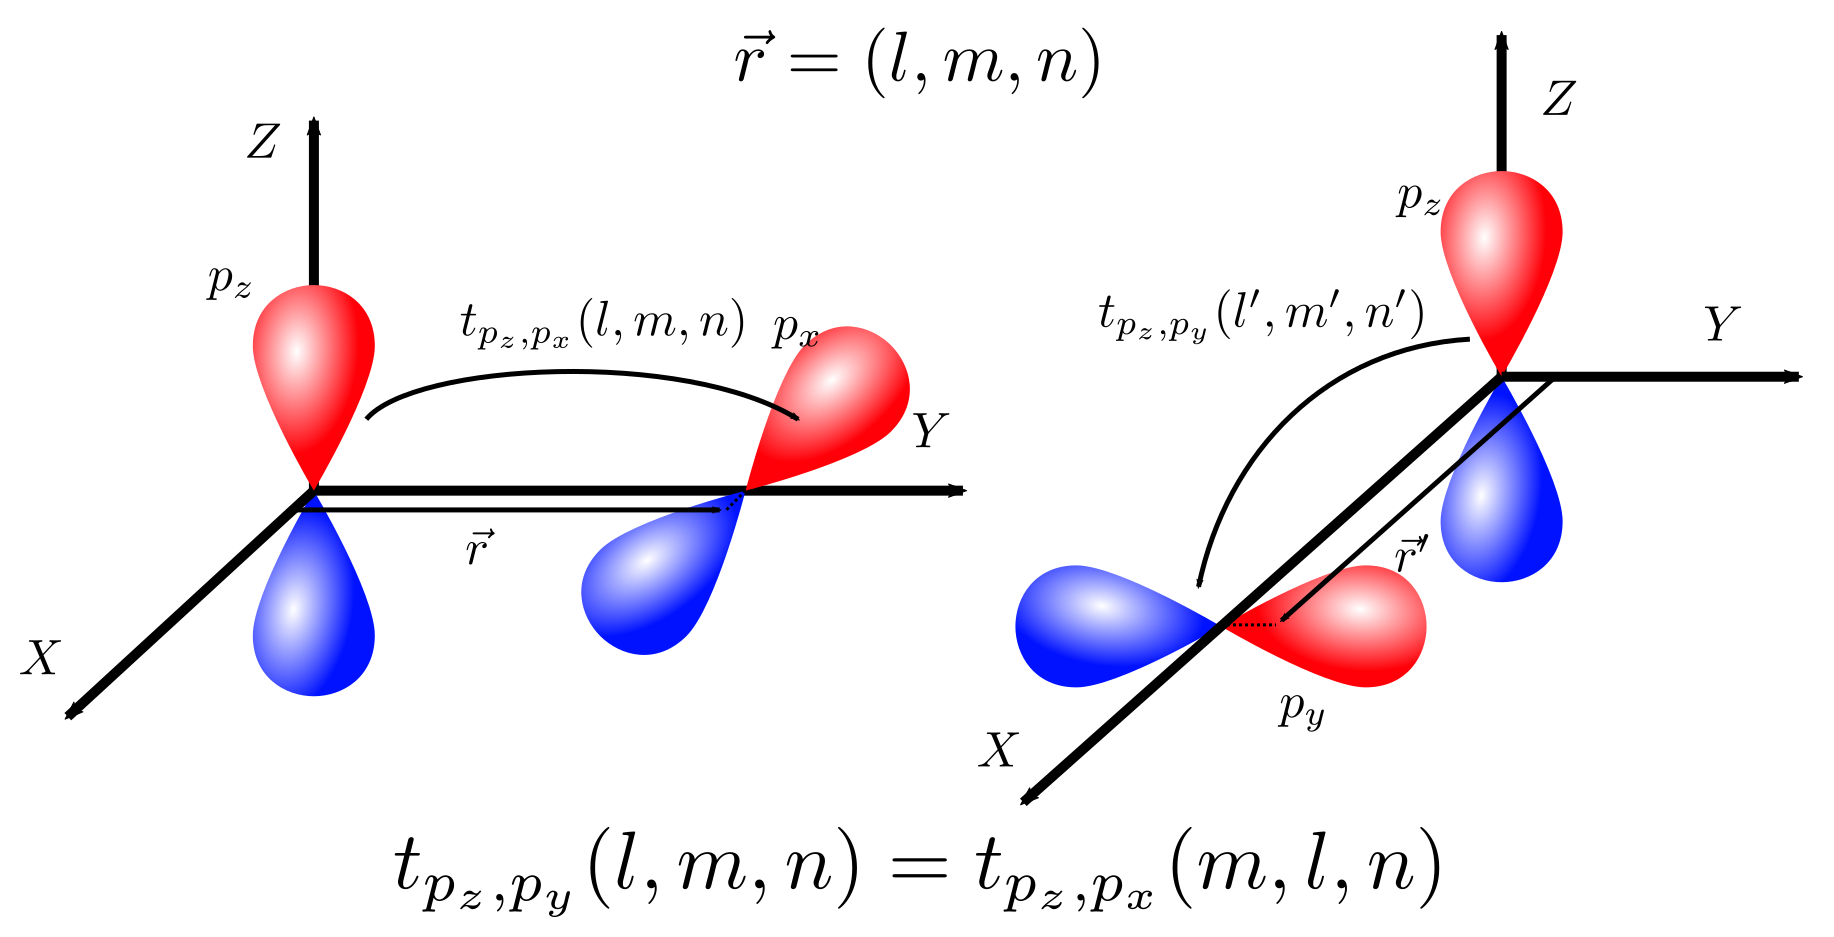
\includegraphics[width=0.45\textwidth]{SK.pdf}
% %   \includegraphics[width=0.45\textwidth]{bilayer_bandDOS.pdf}
% % \vspace{-5pt}
% % \caption{a) Panel show All the possible interlayer hoppings in graphene bilayer. b) Band structure and density of states of graphene bilayer}
% % \label{hoppings}
% % \end{figure}
% % \FloatBarrier
% % %~~~~~~~~~~~~~~~~~~~~~~~~~~~~~~~~~~~~~~~~~~~~~~~~~~~~~~~~~~~%
% \subsection{Electric field}
% % The band structure of graphene bilayer in such a model is shown in \ref{hoppings}.
% The effect of an electric, $\Delta_E$ is to shift the energies of all the orbitals by an amount $\pm\Delta_E$, depending on the layer. This shift opens a gap in the Dirac Points. In nanoislands it can be seen that the gap opens linearly (for low field) with the electric field.
% 
% %~~~~~~~~~~~~~~~~~~~~~~~~~~ FIGURE ~~~~~~~~~~~~~~~~~~~~~~~~~%
% \begin{figure}[h!]
%   \centering
%   \includegraphics[width=\textwidth]{defects/fig/interlayer_elec.pdf}
%   \vspace{-5pt}
% \caption{Evolution of the low energy spectrum (the 8 eigenvalues closest to $E=0$), the hyperfine coupling and the gap with the electric field for different interlayer couplings. In the first panels the blue dots are the spectrum for the pristine island, without $H$ adatom and the red one is the defected case.}
% \label{spectrums}
% \end{figure}
% \FloatBarrier
% %~~~~~~~~~~~~~~~~~~~~~~~~~~~~~~~~~~~~~~~~~~~~~~~~~~~~~~~~~~~%
% 
% Given an island of a certain size (within the shadowed region in Fig.~\ref{confinement}) the evolution of the spectrum is shown in Fig.~\ref{spectrums}, Notice that the figure \emph{does not show bands} but rather discrete spectrums at different electric fields, in particular, the point at $\Delta_E=0$ \emph{is not the Dirac point}, it is simply the spectrum at zero electric field.
% 
% The main information that we can extract by now from Fig.~\ref{spectrums} is that the electronic structure of graphene bilayer opens a gap with the electric field.
% 
% The real value of the interlayer should be the one in the left panel, and it will be the one used from now on, meaning that \emph{the interlayer coupling will not be a free parameter in our calculations}.
% 
% 
% \section{H adatom on graphene bilayer}
% 
% The physics of a $H$ adatom on bilayer graphene does not differ much from the monolayer case. In this case, again the Lieb's theorem nearly applies, although not exactly since the presence of $s$ orbitals break the bipartite character of the system.
% 
% To strictly recover the vacancy limit we would need to freeze the $s-s$ hopping ($V_{ss\sigma}\to0$) and increase the $s-p_z$ ($V_{sp\sigma}\to\infty$) as well as the on-site of the H atom ($\varepsilon_{H_s}\to-\infty$).
% 
% The effect of having finite hoppings and on-site energy is that the ``zero energy'' state is no longer at $E=0$.
% 
% %~~~~~~~~~~~~~~~~~~~~~~~~~~ FIGURE ~~~~~~~~~~~~~~~~~~~~~~~~~%
% \begin{figure}[h!]
%   \centering
%   \includegraphics[width=0.9\textwidth]{defects/fig/parameter_space_bi.pdf}
%   \vspace{-5pt}
% \caption{Parameter space for the energy of the in-gap state and the hyperfine coupling for a graphene bilayer nanoisland.}
% \label{SK2d_bi}
% \end{figure}
% \FloatBarrier
% %~~~~~~~~~~~~~~~~~~~~~~~~~~~~~~~~~~~~~~~~~~~~~~~~~~~~~~~~~~~%
% 
% Notice that the parameter space $V_{ss\sigma}-V_{sp\sigma}$ looks quite similar to the monolayer case (Fig.~\ref{SK2d}) although there is a strong reduction in the hyperfine coupling $\mathcal{A}$ since the in-gap state is extended now among roughly twice as many atoms.\\
% 
% 
% Choosing a value of  $V_{ss\sigma}$, $V_{sp\sigma}$ in the higest region in Fig.~\ref{SK2d_bi} we can see the evolution with the electric field:
% %~~~~~~~~~~~~~~~~~~~~~~~~~~ FIGURE ~~~~~~~~~~~~~~~~~~~~~~~~~%
% \begin{figure}[h!]
%   \centering
%   \includegraphics[width=0.6\textwidth]{defects/fig/best.pdf}
%   \vspace{-5pt}
% \caption{Evolution of the 8 eigenstates closest to $E=0$, the hyperfine coupling and the gap with the electric field}
% \label{best}
% \end{figure}
% \FloatBarrier
% %~~~~~~~~~~~~~~~~~~~~~~~~~~~~~~~~~~~~~~~~~~~~~~~~~~~~~~~~~~~%
% 
% 
% And this is what the hyperfine coupling looks like in the parameter space $V_{ss\sigma}-V_{sp\sigma}$ when the electric field is switched on:
% %~~~~~~~~~~~~~~~~~~~~~~~~~~ FIGURE ~~~~~~~~~~~~~~~~~~~~~~~~~%
% \begin{figure}[h!]
%   \centering
%   \includegraphics{defects/fig/SK_A_bi_e-02.pdf}
%   \vspace{-5pt}
% \caption{Parameter space for the hyperfine coupling for a graphene bilayer nanoisland in the presence of a strong electric field $\Delta_E=-0.2eV$}
% \end{figure}
% \FloatBarrier
% %~~~~~~~~~~~~~~~~~~~~~~~~~~~~~~~~~~~~~~~~~~~~~~~~~~~~~~~~~~~%
